\chapter{Trigger Studies}
\label{chap:TriggerStudies}

\noindent As mentioned in section \ref{sec:TriggerSelection}, for this analysis
the trigger selection was not applied on simulated samples. Instead, it 
was modeled as a weight, which was obtained from the 
trigger efficiency measured with data. The TauPOG (the CMS group dedicated to the tau identification 
criteria) recommends another method to perform the trigger selection. The method
consists in selecting the simulated events that fire the $HLT\_DoubleMediumIsoPFTau35\_Trk1\_eta2p1$
trigger and to apply Data$/$MC scale factors on them. These scale factor were 
measured, by the TauPOG, to match the trigger efficiency curves obtained with simulated samples 
with those obtained with data. The trigger scale factors depend on the tau-\pt~and the decay mode 
\footnote{The trigger efficiency curves are described by a \textit{Cristal Ball function} \cite{bib:TauPOGtriggerEff}, 
where the parameters of those fits depends on the tau-\pt~and on the tau decay mode \cite{bib:TauPOGTriggerSF}}.\\

\noindent The search for \Zprimetotauh~was performed using both
trigger selection methods (the one used in the analysis compared with the one 
recommended by the TauPOG) in order to study their impact on the 
sensitivity. Table \ref{tab:tautriggerappendix} shows the overall yields obtained with 
both methods; the difference between them, for the most considerable backgrounds 
(QCD and DY), is less than 2$\%$, which is within the 
systematic uncertainty associated with the trigger 
selection. Figure \ref{TriggerStudy} shows the significance obtained 
with both methods as a function of the effective visible mass. As can be 
noted in the figure, the significances on the high spectrum 
of the \mass~distribution, where the signal is expected, are 
pretty similar (the difference is $\sim$3$\%$). This means
that, any trigger selection method can be used since 
there is not a considerable impact on the sensitivity of
the search. In order to be consistent with the other 
di-tau channels, the trigger was not applied 
on simulated samples.\\

  \begin{tiny} 
 \begin{table}[ht]
 \centering{ 
  \begin{tabular}{ | l | r | r |} \hline \hline 
 \multicolumn{3}{|c|}{OVERALL YIELDS}  \\ \hline 
 & No trigger applied &  TauPOG recommendation  \\ \hline \hline 
 DY         & 131.61   $\pm$   8.64  & 124.07   $\pm$   8.18 \\ \hline 
 WJets      & 41.91   $\pm$   5.17  & 46.86  $\pm$   5.48   \\ \hline 
 DiBoson    & 3.73   $\pm$   1.07 & 3.98   $\pm$   1.11 \\ \hline 
 \ttbar     & 4.39   $\pm$   1.23 & 5.23   $\pm$   1.35  \\ \hline 
 QCD        & 382.67   $\pm$   24.84 & 381.93   $\pm$   24.95 \\ \hline 
 TOTAL BKG  & 564.30   $\pm$   26.86 & 562.08   $\pm$   26.88  \\ \hline 
 Z$'$3000   & 1.91   $\pm$   0.02  & 1.88   $\pm$   0.02    \\ \hline \hline 
 Significance & 0.34 & 0.33 \\ \hline \hline 
 \end{tabular} 
   }
  \caption{Signal and background yields obtained with trigger selection method used 
  in this analysis and with the one recommended by the TauPOG. The significance was computed for 
  \mass~$>~$600\GeV. \label{tab:tautriggerappendix} }
 \end{table} 
 \end{tiny} 

\begin{figure}[H]
\begin{center}
\captionsetup[subfloat]{farskip=0pt,captionskip=0.0cm,labelformat=empty}
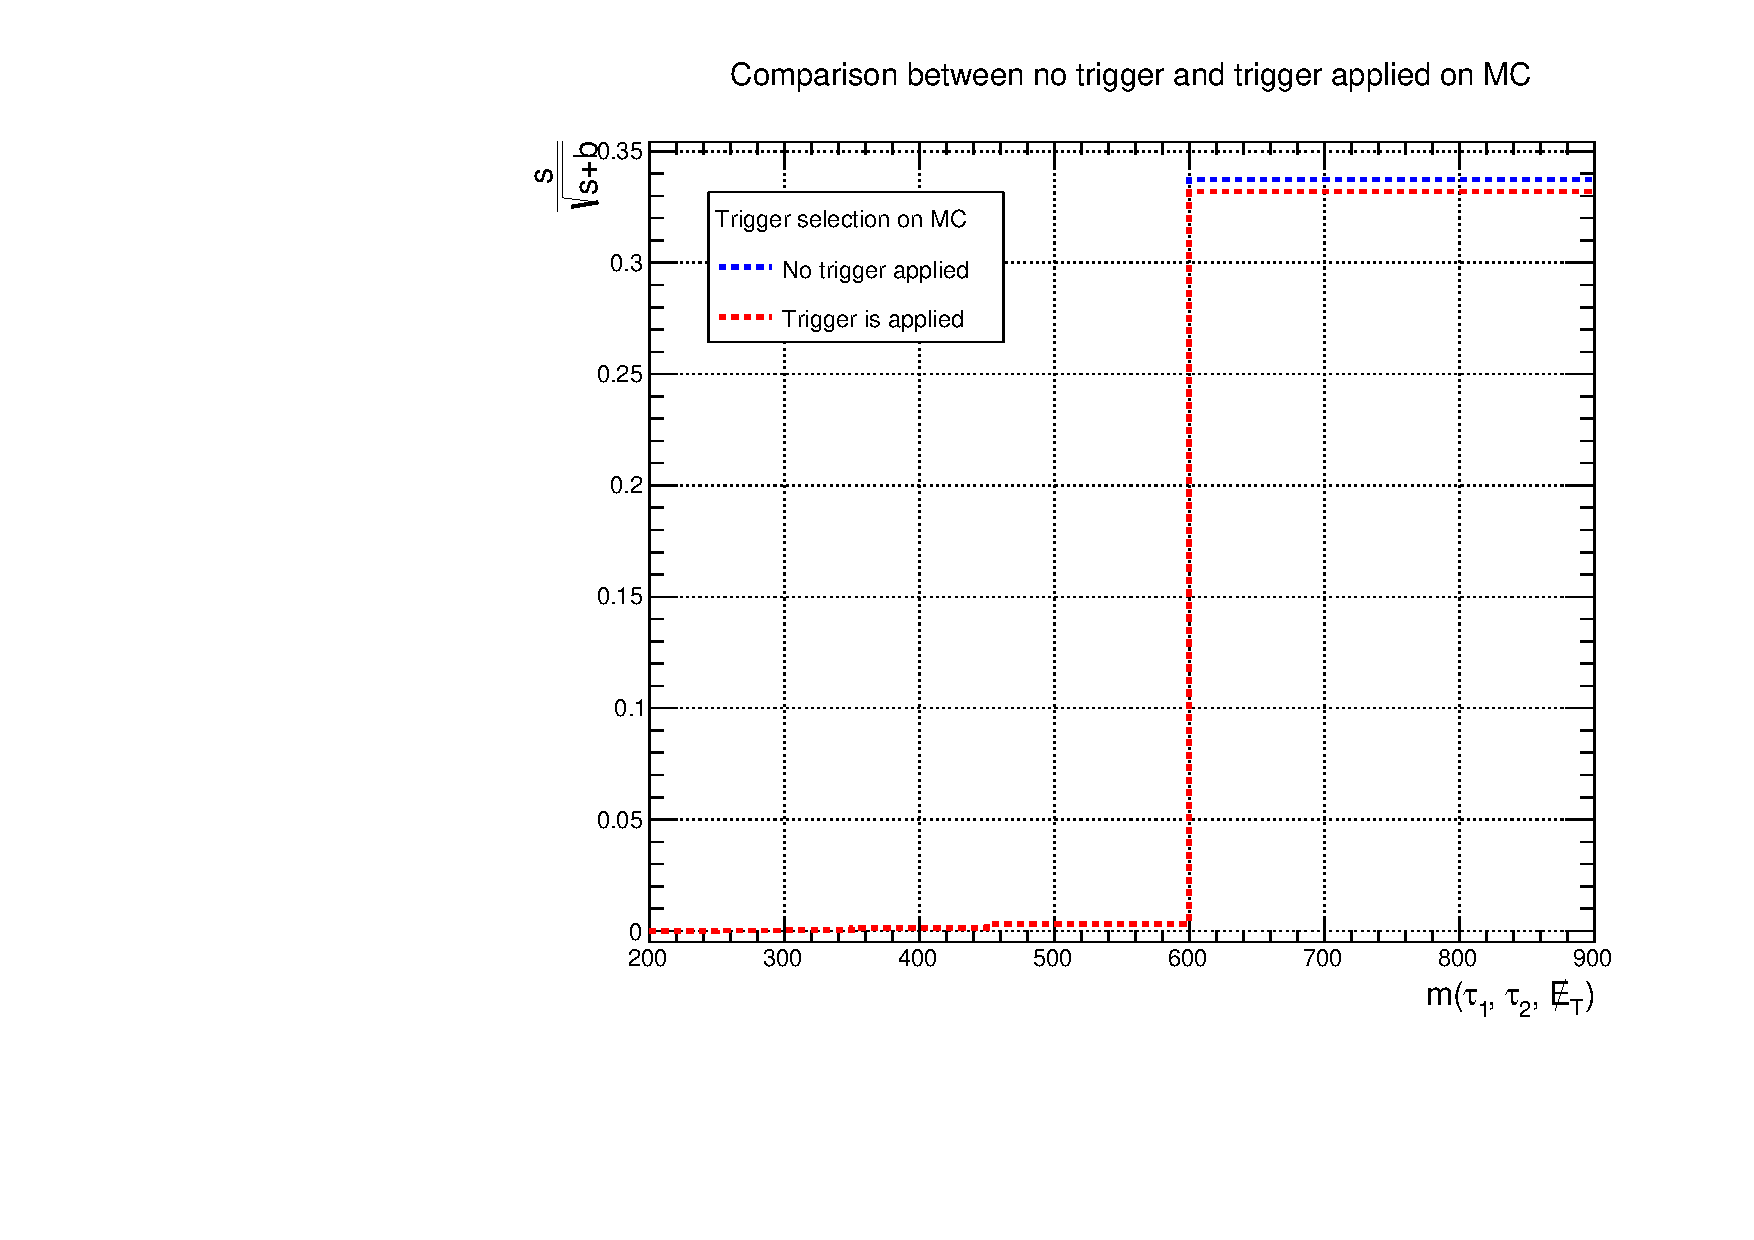
\includegraphics[clip,width=0.5\textwidth]{figuras/AppendiceA/trigger.pdf}
\end{center}
 \caption{Significance, as a function of the effective visible mass, obtained 
 with trigger selection method used in this analysis and with the one 
 recommended by the TauPOG. \label{TriggerStudy}}
\end{figure}

% \begin{equation}
% SF(\textrm{p}_{\textrm{T}}) = \left \{ \begin{matrix} \frac{N}{area} \cdot [1.0 + \mbox{erf}(x)] \cdot \sqrt{\pi/2} & \mbox{if }t \leq \left|\frac{\alpha}{\sigma}\right|
% \\ \\ \frac{N}{area} \cdot \left[L + \frac{a}{1-n} \cdot \left( \left(t-b\right)^{1-n} -\left(\left|\frac{\alpha}{\sigma}\right|-b\right)^{1-n} \right)  \right] & \mbox{if }t > \left|\frac{\alpha}{\sigma}\right| \end{matrix}\right.
% \end{equation}
 